\documentclass[11pt]{article}
\usepackage[margin=1in]{geometry}
\usepackage[T1]{fontenc}
\usepackage{lmodern}
\usepackage{graphicx}
\usepackage{booktabs}
\usepackage{longtable}
\usepackage[table]{xcolor}
\usepackage{amsmath}
\usepackage{amssymb}
\usepackage{float}
\usepackage{listings}
\usepackage{enumitem}
\usepackage{caption}
\usepackage{subcaption}
\usepackage[hidelinks]{hyperref}
\setlist{itemsep=2pt,topsep=3pt}
\lstset{basicstyle=\ttfamily\small,frame=single,columns=fullflexible,breaklines=true}
\emergencystretch=2em
\graphicspath{{../plots/}{figs/}}

\begin{document}
\begin{titlepage}
\centering\vspace*{4cm}
{\LARGE\bfseries Multiclass Classification of Customer Segments\par}\vspace{0.6cm}
{\large Data Analytics 1 --- Assignment 4, Section 1\par}\vspace{0.4cm}
{\large Team: teamId\par}\vspace{1.5cm}
\begin{minipage}{0.8\textwidth}\small\raggedright
Deliverables covered: \texttt{teamId\_classifier\_ovo.py}, \texttt{teamId\_classifier\_ova.py}
(with \texttt{ovo.csv}, \texttt{ova.csv}), \texttt{teamId\_random\_forest.ipynb} (with \texttt{rf.csv}),
\texttt{teamId\_task3\_analysis.ipynb}.
All numbers in this report are taken from the grid-search CSV files, the cached parameter files and
the stored outputs of the two notebooks.
\end{minipage}
\end{titlepage}
\tableofcontents
\newpage

%=====================================================================
\section{Data and Preprocessing}
%=====================================================================
\texttt{Customer\_train.csv} has 1{,}838 labelled customers; \texttt{Customer\_test.csv} has the
789 potential customers without the target. The column \texttt{ID} is an identifier with no
predictive meaning and is dropped. The remaining nine attributes are:

\begin{table}[H]\centering\small
\caption{Attribute types, encoding and number of missing values in the training set.}\label{tab:attrs}
\begin{tabular}{@{}llp{6.2cm}r@{}}
\toprule
Attribute & Type & Treatment & Missing \\
\midrule
Age & numeric & median imputation, standardisation & 0 \\
Work\_Experience & numeric & median imputation, standardisation & 174 \\
Family\_Size & numeric & median imputation, standardisation & 78 \\
Spending\_Score & ordinal & most-frequent imputation, ordinal code Low\,$<$\,Average\,$<$\,High (0,1,2), standardisation & 0 \\
Gender & nominal & most-frequent imputation, one-hot, standardisation & 0 \\
Ever\_Married & nominal & as above & 31 \\
Graduated & nominal & as above & 16 \\
Profession & nominal & as above & 26 \\
Var\_1 & nominal & as above & 22 \\
\bottomrule
\end{tabular}
\end{table}

\paragraph{Leakage-free pipeline.} All preprocessing is a single scikit-learn
\texttt{ColumnTransformer} (imputers; an \texttt{OrdinalEncoder} with the explicit order for
\texttt{Spending\_Score}; a \texttt{OneHotEncoder} with \texttt{handle\_unknown="ignore"}; a
\texttt{StandardScaler})
placed in a \texttt{Pipeline} together with the classifier. During cross-validation the pipeline is
re-fitted on the training folds only, so medians, modes, categories and scaling statistics never see
the validation rows; the final models are fitted on the full training file and only \emph{applied}
to the test file. The random forest notebook imports the very same preprocessor from
\texttt{teamId\_classifier\_ovo.py}. Scaling matters for the RBF/polynomial SVMs; it is harmless for
trees. Unseen test categories are encoded as all-zero one-hot vectors.

\paragraph{Class distribution and imbalance.} The four segments are A 580 (31.6\%), D 547 (29.8\%),
B 391 (21.3\%) and C 320 (17.4\%). The imbalance is moderate, but because the attributes carry
little signal it strongly influences what an unweighted learner predicts (Section~\ref{sec:t3a}).
We handle it in three ways: (i) all CV splits are stratified; (ii) \texttt{class\_weight} (none
vs.\ balanced) is part of the SVM search grid; (iii) every model, including the random forest, is
selected by \emph{macro-F1} rather than accuracy, with accuracy reported alongside.

%=====================================================================
\section{Task 1: One-vs-One and One-vs-All SVMs}
%=====================================================================
\subsection{(a) One-vs-one design}
The class \texttt{OneVsOneSVM} in \texttt{teamId\_classifier\_ovo.py} trains
$\binom{4}{2}=6$ binary \texttt{sklearn.svm.SVC} models, one per pair $(a,b)$, each fitted only on
the rows whose label is $a$ or $b$ (so every SVM sees a binary target). For a test point $x$ the
pairwise SVM returns a signed margin $f_{ab}(x)$, positive in favour of $b$. Prediction:
\begin{enumerate}
\item \textbf{Votes.} Each SVM gives one vote to the winner of its pair; the class with most votes wins.
\item \textbf{Tie on votes $\rightarrow$ summed margins.} Among tied classes, choose the one with the
largest total signed margin $s_c(x)=\sum_{b}f_{bc}(x)-\sum_{b}f_{cb}(x)$, i.e.\ the sum over its
pairwise SVMs of the margin in its favour.
\item \textbf{Still tied $\rightarrow$ training prior.} Choose the class with the larger training frequency.
\item \textbf{Still tied $\rightarrow$ seeded random choice} among the remaining classes (seed 42, reproducible).
\end{enumerate}
\emph{Why this is label-order independent.} Every criterion is a property of the class itself (its
votes, its margins, its frequency); none uses the position of the label in a sorted list, as
\texttt{argmax} over a vote vector would (which silently favours the first label, here A). The
final random draw treats all remaining candidates symmetrically, so no label is systematically
favoured. Exact ties beyond step~2 are essentially impossible because the margins are continuous.

\subsection{(b) One-vs-all design}
\texttt{OneVsAllSVM} in \texttt{teamId\_classifier\_ova.py} trains $K=4$ binary SVCs, the
$k$-th on all rows with target $\mathbb{1}[y=k]$. The predicted class is
$\arg\max_k f_k(x)$ of the decision scores. Exact ties (detected with \texttt{np.isclose}) go to the
larger training prior and then to a seeded random choice, again independent of label order.
With \texttt{class\_weight="balanced"} each one-vs-rest problem is re-weighted, which is exactly
where OvA suffers from imbalance (each binary problem is between 32:68 and 17:83).

\paragraph{Compliance with the rules.} Neither \texttt{OneVsOneClassifier} nor
\texttt{OneVsRestClassifier} is imported, and no SVC is ever given more than two labels, so the
built-in multiclass mode of SVC is never triggered. The OvO code asserts that each pairwise SVM's
positive class is the expected one, so votes and margins are attributed correctly.

\paragraph{How to run.} From \texttt{SECTION-1/}:
\begin{lstlisting}
python teamId_classifier_ovo.py <path_to_test_file>   # writes ovo.csv
python teamId_classifier_ova.py <path_to_test_file>   # writes ova.csv
python teamId_classifier_ova.py <path_to_test_file> --retune   # redo grid search
\end{lstlisting}
Each script loads \texttt{Customer\_train.csv} from its own directory, reads the cached
hyperparameters (\texttt{ovo\_best\_params.json} / \texttt{ova\_best\_params.json}; \texttt{-{}-retune}
reruns the full grid search and rewrites the grid CSV), fits the pipeline on all training rows and
writes a single column \texttt{predicted}, one row per test row in input order. For the 789 test
customers the predicted counts are: OvO A 168, B 215, C 202, D 204; OvA A 217, B 197, C 172, D 203.

\subsection{(c) Hyperparameter selection}
Selection uses stratified 5-fold CV (\texttt{shuffle=True, random\_state=42}) with macro-F1 as the
criterion; accuracy is recorded too. The grid (30 configurations per decomposition) is
\begin{itemize}
\item kernel \texttt{linear}: $C\in\{0.1,1,10\}$;
\item kernel \texttt{rbf}: $C\in\{0.1,1,10\}$, $\gamma\in\{0.01,0.1,1\}$;
\item kernel \texttt{poly} (degree 2, $\gamma=$ \texttt{scale}): $C\in\{0.1,1,10\}$;
\item each crossed with \texttt{class\_weight} $\in\{$none, balanced$\}$.
\end{itemize}
Tables~\ref{tab:gridovo} and~\ref{tab:gridova} list the mean $\pm$ standard deviation over the five
folds (population std, \texttt{np.std}) for every configuration; the selected row is shaded.
\textbf{Both decompositions select} kernel = RBF, $C=1$, $\gamma=0.1$, \texttt{class\_weight =
balanced}: OvO macro-F1 $0.3113\pm0.0304$ (accuracy $0.3156\pm0.0299$), OvA macro-F1
$0.3143\pm0.0306$ (accuracy $0.3188\pm0.0316$).
Across the whole grid macro-F1 varies widely (0.144--0.311 for OvO, 0.247--0.314 for OvA; fold std
0.002--0.044), so the hyperparameters do matter. The \emph{top} of the grid, however, is crowded:
10 of the 30 OvO and 19 of the 30 OvA configurations lie within one fold-std of the best, so the
choice among them is not sharply determined. For example, the best unweighted OvA (RBF, $C=1$,
$\gamma=0.01$) reaches $0.3116\pm0.0171$, with the highest accuracy in the OvA grid (0.3406).
Unweighted configurations generally have higher accuracy but lower macro-F1, because they predict the
large segments A and D more often.

{\small
\setlength{\tabcolsep}{5pt}
\begin{longtable}{@{}lrllrcc@{}}
\caption{OvO SVM: full search grid, 5-fold CV mean $\pm$ std (selected row shaded).}\label{tab:gridovo}\\
\toprule
Kernel & $C$ & $\gamma$ & Degree & Class weight & Macro-F1 & Accuracy \\
\midrule\endfirsthead
\toprule
Kernel & $C$ & $\gamma$ & Degree & Class weight & Macro-F1 & Accuracy \\
\midrule\endhead
\bottomrule\endfoot
linear & 0.1 & -- & -- & none & 0.2156 $\pm$ 0.0112 & 0.3400 $\pm$ 0.0073 \\
linear & 1 & -- & -- & none & 0.2171 $\pm$ 0.0089 & 0.3400 $\pm$ 0.0055 \\
linear & 10 & -- & -- & none & 0.2178 $\pm$ 0.0098 & 0.3411 $\pm$ 0.0065 \\
rbf & 0.1 & 0.01 & -- & none & 0.2089 $\pm$ 0.0115 & 0.3504 $\pm$ 0.0150 \\
rbf & 0.1 & 0.1 & -- & none & 0.1723 $\pm$ 0.0101 & 0.3346 $\pm$ 0.0107 \\
rbf & 0.1 & 1 & -- & none & 0.1441 $\pm$ 0.0022 & 0.3281 $\pm$ 0.0024 \\
rbf & 1 & 0.01 & -- & none & 0.2136 $\pm$ 0.0085 & 0.3422 $\pm$ 0.0123 \\
rbf & 1 & 0.1 & -- & none & 0.2854 $\pm$ 0.0177 & 0.3254 $\pm$ 0.0150 \\
rbf & 1 & 1 & -- & none & 0.2634 $\pm$ 0.0190 & 0.3123 $\pm$ 0.0200 \\
rbf & 10 & 0.01 & -- & none & 0.2503 $\pm$ 0.0179 & 0.3177 $\pm$ 0.0197 \\
rbf & 10 & 0.1 & -- & none & 0.2950 $\pm$ 0.0238 & 0.3118 $\pm$ 0.0229 \\
rbf & 10 & 1 & -- & none & 0.2831 $\pm$ 0.0186 & 0.3090 $\pm$ 0.0182 \\
poly & 0.1 & scale & 2 & none & 0.1935 $\pm$ 0.0091 & 0.3433 $\pm$ 0.0126 \\
poly & 1 & scale & 2 & none & 0.2324 $\pm$ 0.0100 & 0.3248 $\pm$ 0.0117 \\
poly & 10 & scale & 2 & none & 0.2619 $\pm$ 0.0100 & 0.3036 $\pm$ 0.0173 \\
linear & 0.1 & -- & -- & balanced & 0.2739 $\pm$ 0.0165 & 0.2856 $\pm$ 0.0108 \\
linear & 1 & -- & -- & balanced & 0.2751 $\pm$ 0.0144 & 0.2867 $\pm$ 0.0084 \\
linear & 10 & -- & -- & balanced & 0.2776 $\pm$ 0.0116 & 0.2889 $\pm$ 0.0066 \\
rbf & 0.1 & 0.01 & -- & balanced & 0.2391 $\pm$ 0.0157 & 0.2878 $\pm$ 0.0213 \\
rbf & 0.1 & 0.1 & -- & balanced & 0.2620 $\pm$ 0.0191 & 0.3150 $\pm$ 0.0119 \\
rbf & 0.1 & 1 & -- & balanced & 0.2181 $\pm$ 0.0440 & 0.3009 $\pm$ 0.0379 \\
rbf & 1 & 0.01 & -- & balanced & 0.2880 $\pm$ 0.0222 & 0.2965 $\pm$ 0.0207 \\
\rowcolor{gray!20}rbf & 1 & 0.1 & -- & balanced & \textbf{0.3113} $\pm$ 0.0304 & 0.3156 $\pm$ 0.0299 \\
rbf & 1 & 1 & -- & balanced & 0.3023 $\pm$ 0.0179 & 0.3210 $\pm$ 0.0211 \\
rbf & 10 & 0.01 & -- & balanced & 0.2994 $\pm$ 0.0157 & 0.3031 $\pm$ 0.0157 \\
rbf & 10 & 0.1 & -- & balanced & 0.3002 $\pm$ 0.0237 & 0.3041 $\pm$ 0.0244 \\
rbf & 10 & 1 & -- & balanced & 0.2912 $\pm$ 0.0178 & 0.3096 $\pm$ 0.0177 \\
poly & 0.1 & scale & 2 & balanced & 0.2202 $\pm$ 0.0314 & 0.2421 $\pm$ 0.0205 \\
poly & 1 & scale & 2 & balanced & 0.2738 $\pm$ 0.0140 & 0.2748 $\pm$ 0.0142 \\
poly & 10 & scale & 2 & balanced & 0.2872 $\pm$ 0.0120 & 0.2900 $\pm$ 0.0129 \\

\end{longtable}

\begin{longtable}{@{}lrllrcc@{}}
\caption{OvA SVM: full search grid, 5-fold CV mean $\pm$ std (selected row shaded).}\label{tab:gridova}\\
\toprule
Kernel & $C$ & $\gamma$ & Degree & Class weight & Macro-F1 & Accuracy \\
\midrule\endfirsthead
\toprule
Kernel & $C$ & $\gamma$ & Degree & Class weight & Macro-F1 & Accuracy \\
\midrule\endhead
\bottomrule\endfoot
linear & 0.1 & -- & -- & none & 0.2513 $\pm$ 0.0239 & 0.2715 $\pm$ 0.0245 \\
linear & 1 & -- & -- & none & 0.2782 $\pm$ 0.0319 & 0.2932 $\pm$ 0.0300 \\
linear & 10 & -- & -- & none & 0.2539 $\pm$ 0.0223 & 0.2715 $\pm$ 0.0248 \\
rbf & 0.1 & 0.01 & -- & none & 0.2978 $\pm$ 0.0198 & 0.3346 $\pm$ 0.0141 \\
rbf & 0.1 & 0.1 & -- & none & 0.3039 $\pm$ 0.0105 & 0.3254 $\pm$ 0.0162 \\
rbf & 0.1 & 1 & -- & none & 0.2900 $\pm$ 0.0142 & 0.3188 $\pm$ 0.0158 \\
rbf & 1 & 0.01 & -- & none & 0.3116 $\pm$ 0.0171 & 0.3406 $\pm$ 0.0174 \\
rbf & 1 & 0.1 & -- & none & 0.3012 $\pm$ 0.0128 & 0.3210 $\pm$ 0.0170 \\
rbf & 1 & 1 & -- & none & 0.2883 $\pm$ 0.0138 & 0.3167 $\pm$ 0.0129 \\
rbf & 10 & 0.01 & -- & none & 0.2973 $\pm$ 0.0216 & 0.3248 $\pm$ 0.0236 \\
rbf & 10 & 0.1 & -- & none & 0.3022 $\pm$ 0.0188 & 0.3167 $\pm$ 0.0204 \\
rbf & 10 & 1 & -- & none & 0.2847 $\pm$ 0.0213 & 0.3052 $\pm$ 0.0199 \\
poly & 0.1 & scale & 2 & none & 0.2580 $\pm$ 0.0157 & 0.2981 $\pm$ 0.0174 \\
poly & 1 & scale & 2 & none & 0.2660 $\pm$ 0.0200 & 0.3085 $\pm$ 0.0266 \\
poly & 10 & scale & 2 & none & 0.2534 $\pm$ 0.0137 & 0.3003 $\pm$ 0.0176 \\
linear & 0.1 & -- & -- & balanced & 0.2892 $\pm$ 0.0178 & 0.3107 $\pm$ 0.0161 \\
linear & 1 & -- & -- & balanced & 0.2893 $\pm$ 0.0130 & 0.3101 $\pm$ 0.0098 \\
linear & 10 & -- & -- & balanced & 0.2848 $\pm$ 0.0146 & 0.3041 $\pm$ 0.0109 \\
rbf & 0.1 & 0.01 & -- & balanced & 0.2797 $\pm$ 0.0320 & 0.2905 $\pm$ 0.0236 \\
rbf & 0.1 & 0.1 & -- & balanced & 0.2970 $\pm$ 0.0249 & 0.3123 $\pm$ 0.0219 \\
rbf & 0.1 & 1 & -- & balanced & 0.2474 $\pm$ 0.0208 & 0.3177 $\pm$ 0.0146 \\
rbf & 1 & 0.01 & -- & balanced & 0.3038 $\pm$ 0.0137 & 0.3085 $\pm$ 0.0151 \\
\rowcolor{gray!20}rbf & 1 & 0.1 & -- & balanced & \textbf{0.3143} $\pm$ 0.0306 & 0.3188 $\pm$ 0.0316 \\
rbf & 1 & 1 & -- & balanced & 0.2934 $\pm$ 0.0147 & 0.3096 $\pm$ 0.0151 \\
rbf & 10 & 0.01 & -- & balanced & 0.3040 $\pm$ 0.0157 & 0.3052 $\pm$ 0.0157 \\
rbf & 10 & 0.1 & -- & balanced & 0.2987 $\pm$ 0.0142 & 0.3047 $\pm$ 0.0159 \\
rbf & 10 & 1 & -- & balanced & 0.2844 $\pm$ 0.0234 & 0.3036 $\pm$ 0.0229 \\
poly & 0.1 & scale & 2 & balanced & 0.2527 $\pm$ 0.0086 & 0.2568 $\pm$ 0.0076 \\
poly & 1 & scale & 2 & balanced & 0.2802 $\pm$ 0.0102 & 0.2835 $\pm$ 0.0117 \\
poly & 10 & scale & 2 & balanced & 0.2831 $\pm$ 0.0248 & 0.2862 $\pm$ 0.0260 \\

\end{longtable}
}

%=====================================================================
\section{Task 2: Random Forest from Scratch}
%=====================================================================
\subsection{(a) Implementation}
\texttt{ScratchRandomForest} (notebook \texttt{teamId\_random\_forest.ipynb}) implements:
\begin{itemize}
\item \textbf{Bootstrap sampling (own code):} for each tree, $n$ row indices are drawn with replacement
(\texttt{rng.randint(0, n, n)}); the rows never drawn form that tree's out-of-bag set.
\item \textbf{Random feature sub-sampling at every split:} each tree is a scikit-learn decision tree
(\texttt{DecisionTreeClassifier}) with \texttt{max\_features="sqrt"}, which draws a fresh random subset of
$\lfloor\sqrt{p}\rfloor$ features at \emph{each node}, not once per tree.
\item \textbf{Aggregation (own code):} majority vote over trees; vote ties go to the larger training
prior and then to a seeded random choice (the same order-independent rule as the SVMs).
\item \textbf{OOB estimate (own code):} each training row is predicted by a vote of only the trees
for which it was out-of-bag; the OOB accuracy is computed over rows that were OOB at least once.
\end{itemize}
\texttt{RandomForestClassifier}, \texttt{ExtraTreesClassifier} and \texttt{BaggingClassifier} are not
used. The model is wrapped with the same preprocessing pipeline as the SVMs.

\begin{table}[H]\centering\small
\caption{Which part of the forest is implemented where.}\label{tab:rfparts}
\begin{tabular}{@{}lp{10.2cm}@{}}
\toprule
Component & Implementation \\
\midrule
Bootstrap sampling of rows & \textbf{Own code}: $n$ indices drawn with replacement per tree \\
Feature sub-sampling at every split & Inside each tree's split search: \texttt{max\_features="sqrt"} draws a new random subset of $\lfloor\sqrt{p}\rfloor$ features at \emph{every node}; each tree receives its own seed from our random generator \\
Aggregation of predictions & \textbf{Own code}: majority vote with an explicit tie rule \\
Out-of-bag estimate & \textbf{Own code}: each row is voted on only by trees that did not see it \\
\bottomrule
\end{tabular}
\end{table}
The assignment allows scikit-learn for the decision trees. Per-split sampling has to happen inside the
tree's split search, because that is the only place where a new subset can be drawn at every node. So
the forest uses the tree's \texttt{max\_features} option for it, while everything that makes the
ensemble a random forest (resampling, seeding, voting, OOB) is our own code.

\subsection{(b) Number of trees and depth}
We tried $n\in\{1,5,10,25,50,100,200\}$ for \texttt{max\_depth} $\in\{4, 8, \text{None}\}$
(Table~\ref{tab:sweep}, Figure~\ref{fig:ntrees}).

\begin{table}[H]\centering\small
\caption{RF sweep: OOB accuracy (full training set) and 5-fold CV accuracy / macro-F1 (mean $\pm$ std).}\label{tab:sweep}
\begin{tabular}{@{}rrccc@{}}
\toprule
max\_depth & $n$ & OOB acc & CV acc & CV macro-F1 \\
\midrule
4 & 1 & 0.3243 & $0.3188\pm0.0291$ & $0.2358\pm0.0307$ \\
4 & 5 & 0.3402 & $0.3390\pm0.0242$ & $0.2202\pm0.0130$ \\
4 & 10 & 0.3407 & $0.3477\pm0.0205$ & $0.2142\pm0.0155$ \\
4 & 25 & 0.3460 & $0.3498\pm0.0088$ & $0.2133\pm0.0049$ \\
4 & 50 & 0.3466 & $0.3493\pm0.0100$ & $0.2131\pm0.0069$ \\
4 & 100 & 0.3487 & $0.3504\pm0.0099$ & $0.2144\pm0.0053$ \\
4 & 200 & 0.3498 & $0.3509\pm0.0112$ & $0.2160\pm0.0067$ \\
\midrule
8 & 1 & 0.2731 & $0.2982\pm0.0127$ & $0.2578\pm0.0240$ \\
8 & 5 & 0.3123 & $0.3297\pm0.0205$ & $0.2562\pm0.0163$ \\
8 & 10 & 0.3308 & $0.3449\pm0.0135$ & $0.2672\pm0.0273$ \\
8 & 25 & 0.3210 & $0.3471\pm0.0160$ & $0.2650\pm0.0300$ \\
8 & 50 & 0.3324 & $0.3493\pm0.0146$ & $0.2647\pm0.0208$ \\
8 & 100 & 0.3400 & $0.3460\pm0.0022$ & $0.2593\pm0.0115$ \\
8 & 200 & 0.3395 & $0.3509\pm0.0092$ & $0.2670\pm0.0108$ \\
\midrule
None & 1 & 0.2731 & $0.2927\pm0.0066$ & $0.2832\pm0.0065$ \\
None & 5 & 0.3002 & $0.3052\pm0.0247$ & $0.2821\pm0.0183$ \\
None & 10 & 0.2951 & $0.3047\pm0.0129$ & $0.2852\pm0.0163$ \\
None & 25 & 0.3090 & $0.3128\pm0.0128$ & $0.2937\pm0.0159$ \\
None & 50 & 0.3128 & $0.3221\pm0.0154$ & $0.3048\pm0.0197$ \\
None & 100 & 0.3128 & $0.3199\pm0.0120$ & $0.3029\pm0.0186$ \\
\rowcolor{gray!20}None & 200 & 0.3161 & $0.3254\pm0.0148$ & $0.3109\pm0.0221$ \\
\bottomrule
\end{tabular}
\end{table}

\begin{figure}[H]\centering
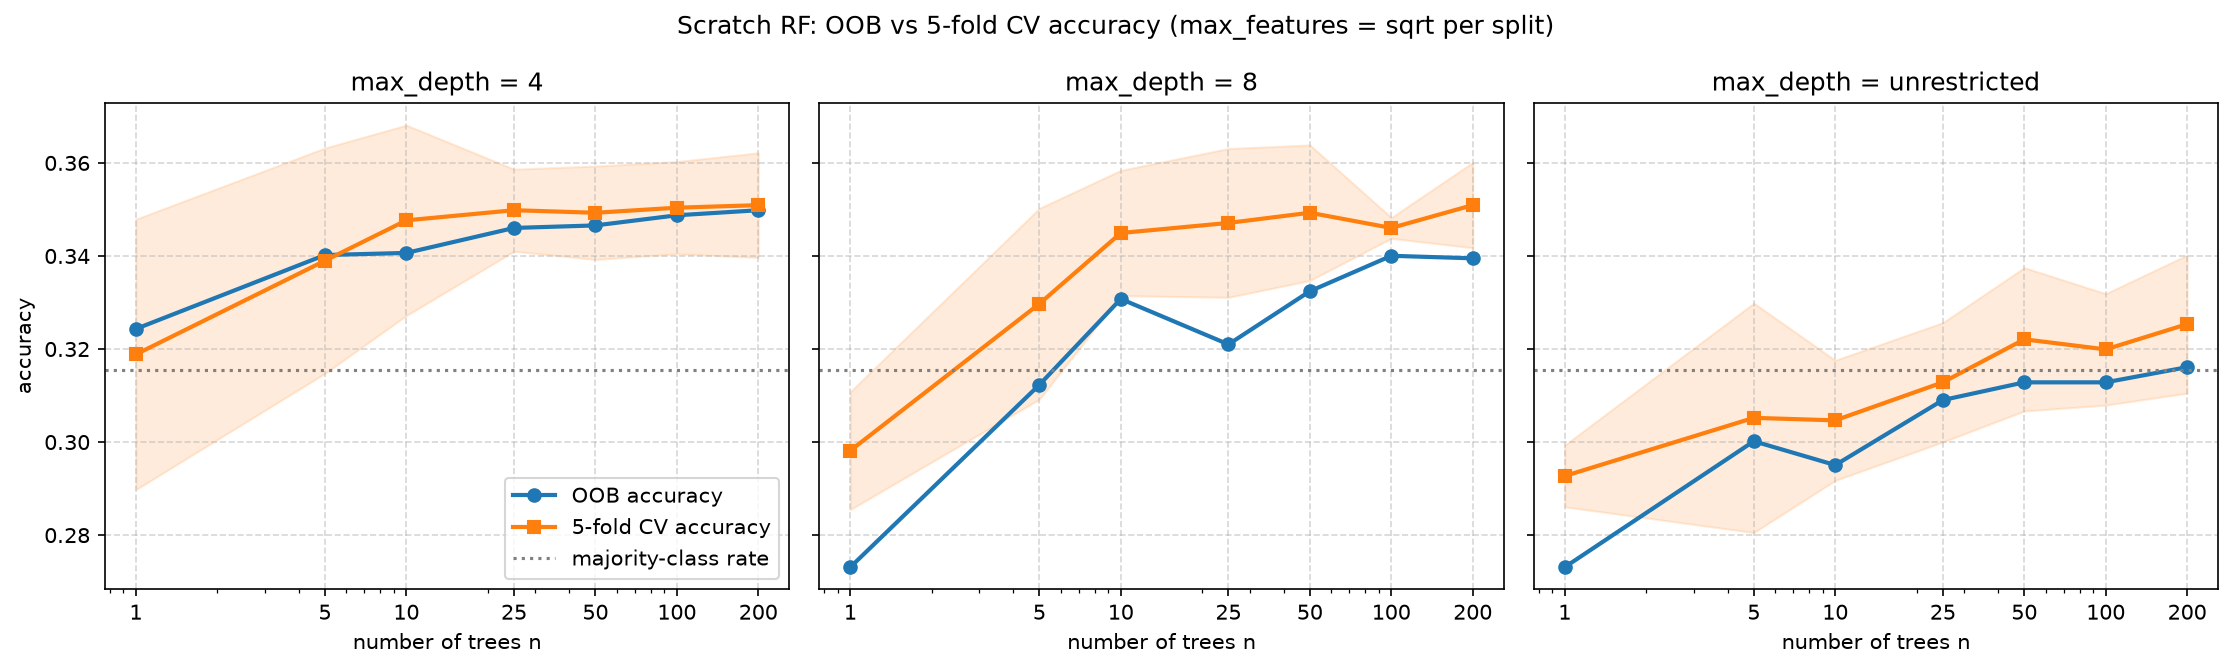
\includegraphics[width=\textwidth]{rf_accuracy_vs_ntrees.png}
\caption{OOB and 5-fold CV accuracy versus number of trees (log scale) for three depths; band = CV
$\pm1$ std, dotted line = majority-class rate 0.316.}\label{fig:ntrees}
\end{figure}

\paragraph{Shape of the curves.}
\begin{itemize}
\item \textbf{Rapid rise, then plateau.} A single tree is a noisy, high-variance classifier (CV accuracy
0.319, 0.298, 0.293 for depth 4, 8, unrestricted). Averaging decorrelated trees reduces the variance
of the vote, so accuracy climbs quickly up to $n\approx10$--25 and then flattens: from $n=50$ to
$200$ the CV accuracy changes by only $+0.0016$, $+0.0016$ and $+0.0033$, all below the fold std.
More trees do not overfit; they simply stop helping.
\item \textbf{Depth matters more than $n$.} Depth-4 forests plateau near 0.35 accuracy, unrestricted forests
at 0.293--0.325: deep trees fit noise in their bootstrap sample and averaging only partly cancels it.
\item \textbf{Accuracy vs.\ macro-F1 move in opposite directions.} Shallow forests obtain their accuracy by
predicting mostly A and D (macro-F1 0.213--0.236 at depth 4), whereas unrestricted forests predict
all four segments (macro-F1 0.282--0.311).
\item \textbf{OOB vs.\ CV.} OOB tracks CV closely but sits slightly below it (chosen model: OOB 0.3161
vs.\ CV 0.3254). Each tree leaves out about 36.8\% of the rows, so every row's OOB prediction is a vote
of only $\approx$37\% of the trees, a smaller and weaker forest than the full one. This makes OOB slightly
pessimistic, most visibly at small $n$, where a row is out-of-bag for very few trees.
\end{itemize}

\paragraph{Chosen configuration.} Selecting by CV macro-F1 (ties to fewer trees), the same criterion as
for the SVMs, gives $n=200$, \texttt{max\_depth = None} (saved in \texttt{rf\_best\_params.json}):
CV macro-F1 $0.3109\pm0.0221$, CV accuracy $0.3254\pm0.0148$, OOB accuracy 0.3161. Selecting by
accuracy would instead pick a depth-4 or depth-8 forest (CV accuracy 0.3509) that almost never
predicts B or C (macro-F1 0.216--0.267).

\subsection{(c) Metrics and test predictions}
Table~\ref{tab:rfmetrics} reports metrics from the pooled 5-fold out-of-fold predictions and from the
OOB predictions of the final model.

\begin{table}[H]\centering\small
\caption{Random forest ($n=200$, unrestricted depth): per-class metrics.}\label{tab:rfmetrics}
\begin{tabular}{@{}lccccccr@{}}
\toprule
& \multicolumn{3}{c}{5-fold CV (out-of-fold)} & \multicolumn{3}{c}{OOB} & \\
\cmidrule(lr){2-4}\cmidrule(lr){5-7}
Class & Precision & Recall & F1 & Precision & Recall & F1 & Support \\
\midrule
A & 0.3364 & 0.3759 & 0.3550 & 0.3338 & 0.3793 & 0.3551 & 580 \\
B & 0.2702 & 0.2481 & 0.2587 & 0.2535 & 0.2302 & 0.2413 & 391 \\
C & 0.2953 & 0.2344 & 0.2613 & 0.2773 & 0.2219 & 0.2465 & 320 \\
D & 0.3605 & 0.3803 & 0.3701 & 0.3521 & 0.3656 & 0.3587 & 547 \\
\midrule
Accuracy & \multicolumn{3}{c}{0.3254} & \multicolumn{3}{c}{0.3161} & 1838 \\
Macro-F1 & \multicolumn{3}{c}{0.3113} & \multicolumn{3}{c}{0.3004} & \\
Weighted-F1 & \multicolumn{3}{c}{0.3227} & \multicolumn{3}{c}{0.3131} & \\
\bottomrule
\end{tabular}
\end{table}

The OOB numbers are slightly lower than CV; since depth and $n$ were chosen on the same CV folds, the
CV figures carry a small selection optimism and OOB is a nearly independent check.
The final forest, fitted on all 1{,}838 rows, predicts for the 789 test customers
\textbf{A 302, B 161, C 93, D 233}. The full list of predictions is printed in the notebook and saved
as \texttt{rf.csv} (column \texttt{predicted}).

\subsection{(d) Permutation feature importance}
The forest was refitted on a stratified 75\% split and evaluated on the 25\% hold-out (459 rows;
accuracy 0.3087, macro-F1 0.2966). Each \emph{raw} attribute was permuted 30 times (one-hot groups
are permuted as one attribute).

\begin{figure}[H]\centering
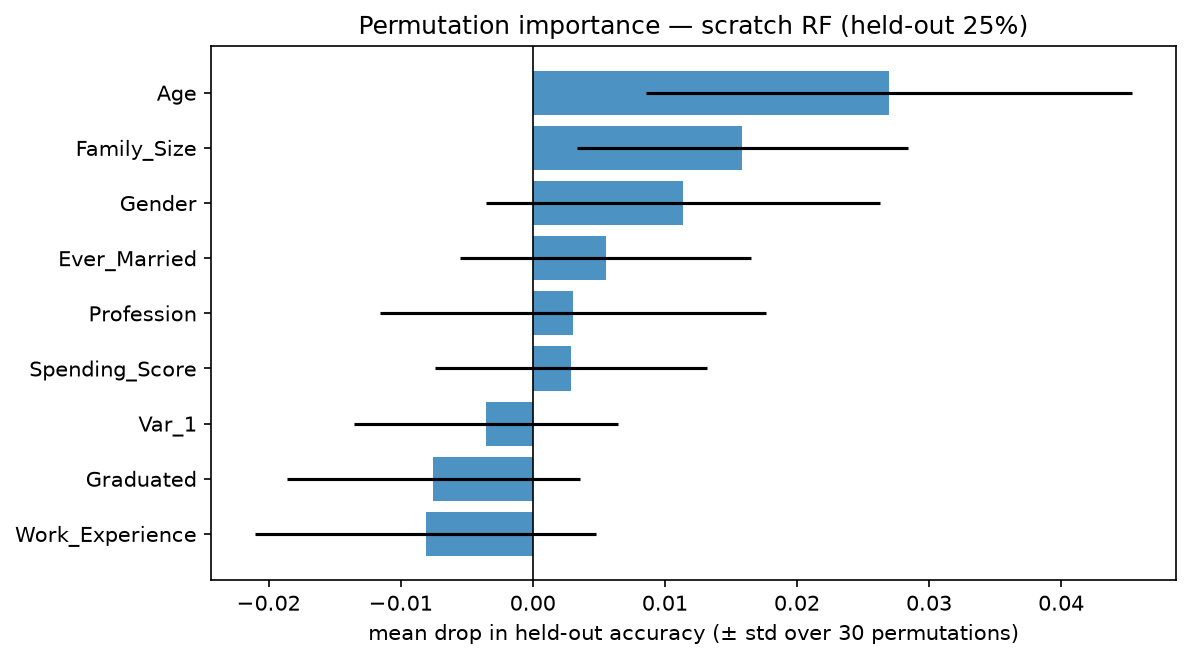
\includegraphics[width=0.85\textwidth]{rf_feature_importance.png}
\caption{Permutation importance on the held-out 25\% (mean drop over 30 permutations, error bars = std).}\label{fig:pi}
\end{figure}

\begin{table}[H]\centering\small
\caption{Permutation importance (mean $\pm$ std drop over 30 shuffles).}\label{tab:pi}
\begin{tabular}{@{}lcc@{}}
\toprule
Attribute & Accuracy drop & Macro-F1 drop \\
\midrule
Age & $0.0270\pm0.0184$ & $0.0402\pm0.0194$ \\
Family\_Size & $0.0159\pm0.0125$ & $0.0180\pm0.0129$ \\
Gender & $0.0114\pm0.0149$ & $0.0233\pm0.0153$ \\
Ever\_Married & $0.0055\pm0.0110$ & $0.0066\pm0.0107$ \\
Profession & $0.0030\pm0.0146$ & $0.0145\pm0.0150$ \\
Spending\_Score & $0.0029\pm0.0103$ & $0.0041\pm0.0110$ \\
Var\_1 & $-0.0036\pm0.0100$ & $0.0045\pm0.0108$ \\
Graduated & $-0.0075\pm0.0111$ & $-0.0020\pm0.0111$ \\
Work\_Experience & $-0.0081\pm0.0129$ & $-0.0030\pm0.0124$ \\
\bottomrule
\end{tabular}
\end{table}

\paragraph{Which attributes drive the segmentation?} \textbf{Age} and \textbf{Family\_Size} are the only
two attributes whose mean $\pm1$ std accuracy drop excludes zero: Age $0.027\pm0.018$ (1.47 std; macro-F1
drop $0.040\pm0.019$) and Family\_Size $0.016\pm0.013$ (1.27 std). Gender follows (0.77 std in accuracy,
although its macro-F1 drop of $0.023\pm0.015$ is larger); Ever\_Married, Profession and
Spending\_Score are inside the noise, and Var\_1, Graduated and Work\_Experience have negative mean
drops (no usable signal). The std reflects only the shuffles of one hold-out set, so it understates
the true uncertainty, and the ranking below the top two or three would likely change with another split.

\paragraph{Business sense.} Age and household size reflecting life stage is plausible: they shape
what kind of car a customer buys and how a sales team would group them. A gender effect is weak and
should not drive targeting. It is less intuitive that Spending\_Score, Profession and
Work\_Experience add almost nothing, suggesting the sales team's segments were not defined mainly by
these fields (or that their information overlaps with Age). Even Age is worth under 3 points of
accuracy, so the attributes in this file explain little of the segmentation.

%=====================================================================
\section{Task 3: Report and Analysis}
%=====================================================================
All three models (with the hyperparameters chosen above) are evaluated on the \emph{same}
stratified 5-fold split (\texttt{shuffle=True}, \texttt{random\_state=42}), with preprocessing refitted inside each
fold; their out-of-fold (OOF) predictions are pooled over all 1{,}838 rows (Table~\ref{tab:overall}; mF1/wF1 = macro/weighted F1).
Because hyperparameters were chosen on these folds, the CV numbers carry a small optimistic bias (nested
CV would remove it).

\begin{table}[H]\centering\small
\caption{Overall comparison on identical 5-fold CV splits. The mean $\pm$ std columns average the five per-fold scores; the OOF columns are computed once on the pooled out-of-fold predictions of all 1{,}838 rows.}\label{tab:overall}
\setlength{\tabcolsep}{4pt}
\begin{tabular}{@{}lccccc@{}}
\toprule
Model & Acc (mean $\pm$ std) & Macro-F1 (mean $\pm$ std) & OOF acc & OOF mF1 & OOF wF1 \\
\midrule
OvO SVM & $0.3156\pm0.0299$ & $0.3113\pm0.0304$ & 0.3156 & 0.3117 & 0.3178 \\
OvA SVM & $0.3188\pm0.0316$ & $0.3143\pm0.0306$ & 0.3188 & 0.3144 & 0.3208 \\
Random forest & $0.3254\pm0.0148$ & $0.3109\pm0.0221$ & 0.3254 & 0.3113 & 0.3227 \\
\bottomrule
\end{tabular}
\end{table}

\subsection{(a) Class imbalance}\label{sec:t3a}
\paragraph{Effect on multiclass classification.} A learner that minimises 0/1 (or hinge) loss is pulled
toward the frequent classes; when the features are weak, as here, this pull dominates and minority
classes are rarely predicted. Accuracy then looks acceptable while minority recall collapses. The RF
sweep shows it: the forest with the best CV accuracy (depth 8, $n=200$, 0.351) rarely predicts B or C
(recall 0.110 and 0.038),\footnote{Out-of-fold recalls of the depth-8 and depth-4 forests ($n=200$, same
folds), printed by the cell after the imbalance experiment in \texttt{teamId\_task3\_analysis.ipynb}. The depth-4 forest, which ties at 0.351
accuracy, never predicts B or C at all (recall A 0.741, B 0, C 0, D 0.393; macro-F1 0.216).} whereas the macro-F1-selected forest has accuracy 0.325 but recall A 0.376,
B 0.248, C 0.234, D 0.380.

\paragraph{Interaction with one-vs-all.} In OvA each binary problem is ``one class vs.\ the other three'',
so even the largest class is a 32:68 minority and C is 17:83. An unweighted SVM can lower its loss by
pushing points to the ``rest'' side, shrinking the scores of small classes, so the argmax rarely
selects them. OvO trains each SVM on two classes with a much milder skew (at most $580:320\approx1.8:1$),
so one would expect OvA to be the more imbalance-sensitive decomposition.

\paragraph{Experiment.} Same folds and kernel/$C$/$\gamma$; only \texttt{class\_weight} changes
(Table~\ref{tab:imb}, Figure~\ref{fig:imb}).

\begin{table}[H]\centering\small
\caption{Effect of balanced class weights (pooled 5-fold OOF).}\label{tab:imb}
\begin{tabular}{@{}lcccccccccc@{}}
\toprule
& & & \multicolumn{4}{c}{Recall} & \multicolumn{4}{c}{Share of predictions} \\
\cmidrule(lr){4-7}\cmidrule(lr){8-11}
Model & Acc & Macro-F1 & A & B & C & D & A & B & C & D \\
\midrule
OvA, none & 0.321 & 0.301 & 0.388 & 0.212 & 0.209 & 0.393 & 0.374 & 0.165 & 0.132 & 0.328 \\
OvO, none & 0.325 & 0.286 & 0.474 & 0.164 & 0.131 & 0.397 & 0.463 & 0.135 & 0.079 & 0.323 \\
OvA, balanced & 0.319 & 0.314 & 0.284 & 0.330 & 0.303 & 0.356 & 0.258 & 0.263 & 0.208 & 0.270 \\
OvO, balanced & 0.316 & 0.312 & 0.250 & 0.299 & 0.353 & 0.375 & 0.223 & 0.256 & 0.254 & 0.267 \\
\bottomrule
\end{tabular}
\end{table}

\begin{figure}[H]\centering
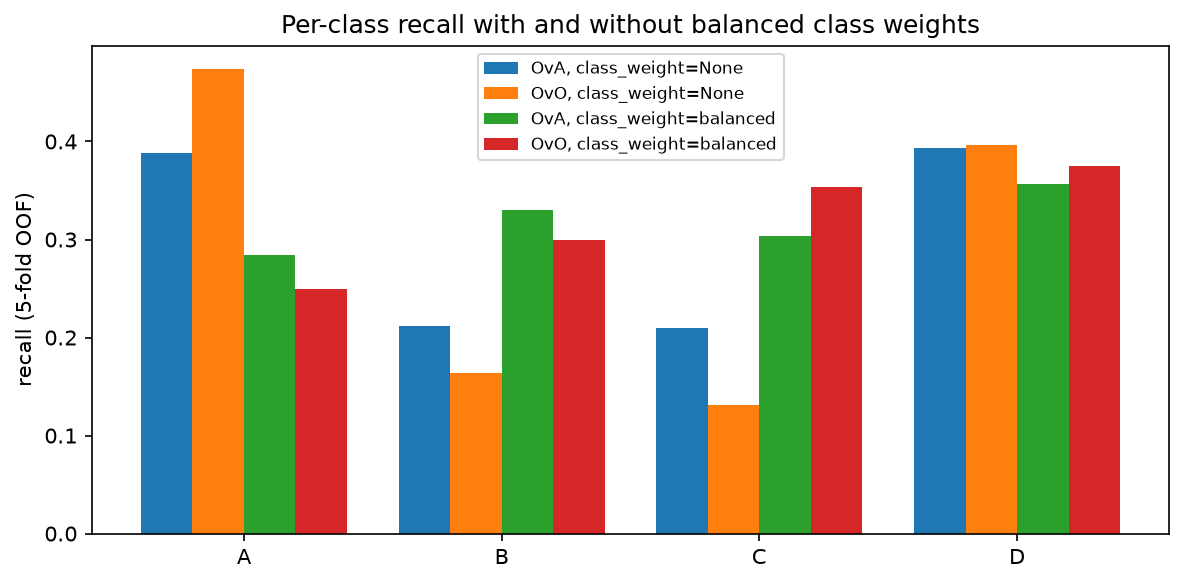
\includegraphics[width=0.85\textwidth]{class_imbalance_experiment.png}
\caption{Per-class recall with and without balanced class weights (5-fold OOF).}\label{fig:imb}
\end{figure}

Without weights both decompositions under-predict the minority classes (true shares: B 21.3\%,
C 17.4\%). Contrary to the theoretical expectation, the unweighted \emph{OvO} is the more skewed one
here: it predicts C for only 7.9\% of rows (recall 0.131, macro-F1 0.286), whereas unweighted OvA
predicts C for 13.2\% (recall 0.209, macro-F1 0.301). The decomposition argument is therefore at
most a tendency on this data. The clear effect of balanced weights is a \emph{shift in recall}: B and C
recall rise by 0.09--0.22 while A recall falls (OvO 0.474$\to$0.250, OvA 0.388$\to$0.284), at a cost of
less than 0.01 in accuracy. The macro-F1 gain is smaller and less certain: a paired bootstrap over rows
(2{,}000 resamples, Task-3 notebook) gives OvA $+0.0130$ [95\% CI $-0.0060$, $+0.0322$], which is
\emph{not} significant, and OvO $+0.0253$ [$+0.0045$, $+0.0440$], which is. Re-weighting therefore reliably
rebalances \emph{which} segments are predicted, and improves macro-F1 significantly only for OvO.

\paragraph{Mitigation strategies, especially for small datasets.}
\begin{itemize}
\item class weights / cost-sensitive loss (no new data needed; used here);
\item selecting models by macro-F1 or balanced accuracy instead of accuracy (used here);
\item stratified CV so every fold contains every class (used here);
\item adjusting decision thresholds, or rescaling OvA scores by class priors;
\item careful oversampling (random oversampling or SMOTE) done \emph{inside} the training folds only;
\item simpler, more regularised models, and collecting more minority-class examples.
\end{itemize}
On small datasets heavy resampling mostly duplicates noise, so re-weighting combined with an
imbalance-aware selection metric is usually the safest choice.

\subsection{(b) Hyperparameters, over- and under-fitting}
\paragraph{SVM.}
\begin{itemize}
\item $C$ trades margin width against training errors. Large $C$ penalises every violation heavily and
fits the training set closely (overfitting); small $C$ gives a wide, soft margin that may ignore real
structure (underfitting).
\item $\gamma$ (RBF width). Large $\gamma$ makes each support vector influence only a tiny neighbourhood,
so the boundary can wrap around individual points (overfitting); small $\gamma$ makes the kernel
nearly linear and the model too smooth (underfitting).
\item Kernel. Flexibility grows from linear to polynomial to RBF; a more flexible kernel lowers bias
but needs stronger regularisation ($C$, $\gamma$) to avoid overfitting.
\end{itemize}
\paragraph{Random forest.}
\begin{itemize}
\item Number of trees: more trees lower the variance of the vote and do \emph{not} cause overfitting;
too few trees give a noisy, high-variance model. Beyond the plateau they only cost time.
\item \texttt{max\_depth}: deep trees have low bias and high variance (each can memorise its bootstrap
sample); very shallow trees underfit.
\item \texttt{min\_samples\_leaf}: small leaves (e.g.\ 1) allow memorisation of single rows (overfitting);
large leaves smooth predictions and can underfit.
\item \texttt{max\_features}: small values decorrelate trees (lower ensemble variance) but raise each
tree's bias; using all features turns the forest into plain bagging with correlated trees, which
averaging helps less.
\end{itemize}

\begin{figure}[H]\centering
\begin{subfigure}{0.49\textwidth}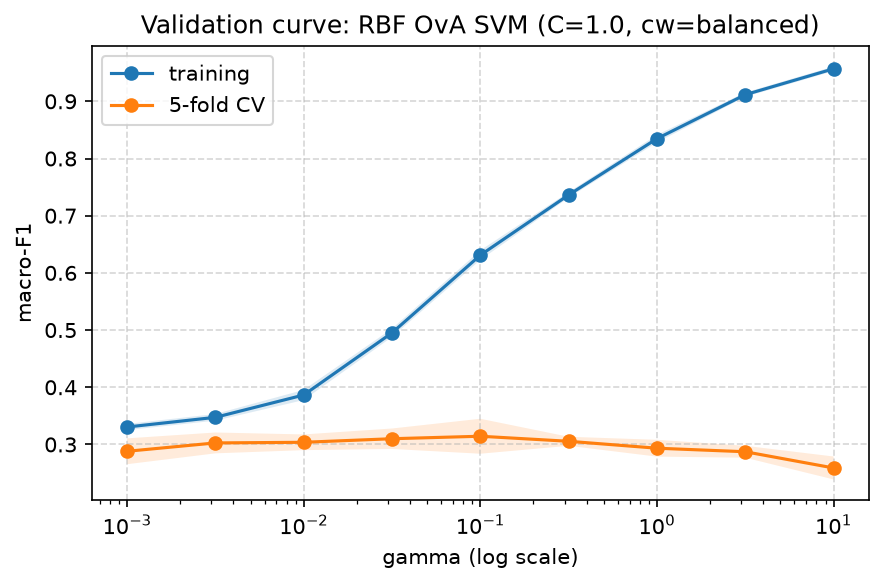
\includegraphics[width=\linewidth]{val_curve_gamma.png}
\caption{OvA SVM, $C=1$, balanced; macro-F1 vs.\ $\gamma$.}\end{subfigure}\hfill
\begin{subfigure}{0.49\textwidth}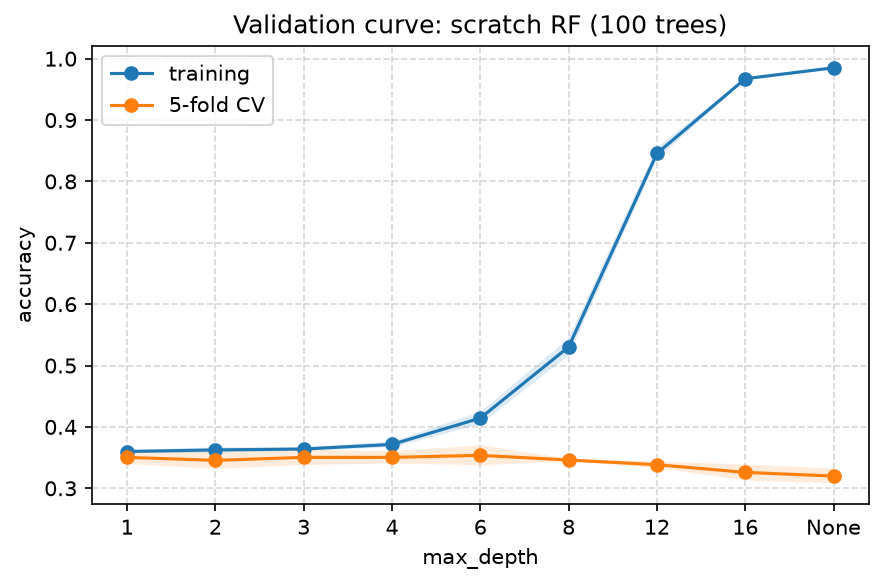
\includegraphics[width=\linewidth]{val_curve_maxdepth.png}
\caption{Scratch RF, 100 trees; accuracy vs.\ max\_depth.}\end{subfigure}

\medskip
\begin{subfigure}{0.49\textwidth}\IfFileExists{../plots/val_curve_maxdepth_f1.png}{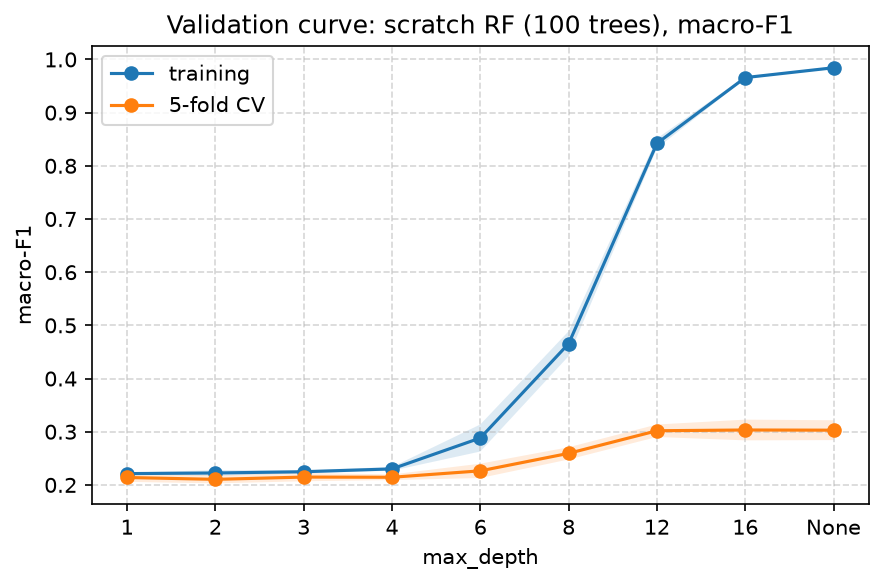
\includegraphics[width=\linewidth]{val_curve_maxdepth_f1.png}}{\fbox{\parbox[c][3cm][c]{0.9\linewidth}{\centering re-run teamId\_task3\_analysis.ipynb to create val\_curve\_maxdepth\_f1.png}}}
\caption{Scratch RF, 100 trees; macro-F1 vs.\ max\_depth.}\end{subfigure}
\caption{Validation curves (training vs.\ 5-fold CV score on the common folds).}\label{fig:vc}
\end{figure}

\begin{table}[H]\centering\small
\caption{Validation-curve values. Left: OvA SVM vs.\ $\gamma$ (macro-F1). Right: RF vs.\ depth.}\label{tab:vc}
\begin{tabular}{@{}rccc@{}}
\toprule
$\gamma$ & Train & CV & CV std \\
\midrule
0.0010 & 0.3305 & 0.2880 & 0.0226 \\
0.0032 & 0.3474 & 0.3027 & 0.0182 \\
0.0100 & 0.3865 & 0.3038 & 0.0137 \\
0.0316 & 0.4952 & 0.3100 & 0.0179 \\
0.1000 & 0.6310 & 0.3143 & 0.0306 \\
0.3162 & 0.7363 & 0.3055 & 0.0079 \\
1.0000 & 0.8347 & 0.2934 & 0.0147 \\
3.1623 & 0.9117 & 0.2872 & 0.0104 \\
10.0000 & 0.9569 & 0.2589 & 0.0200 \\
\bottomrule
\end{tabular}\quad
\begin{tabular}{@{}rcccc@{}}
\toprule
Depth & Train acc & CV acc & Train mF1 & CV mF1 \\
\midrule
1 & 0.3599 & 0.3504 & 0.2212 & 0.2139 \\
2 & 0.3625 & 0.3455 & 0.2224 & 0.2104 \\
3 & 0.3640 & 0.3504 & 0.2247 & 0.2147 \\
4 & 0.3715 & 0.3504 & 0.2301 & 0.2144 \\
6 & 0.4143 & 0.3537 & 0.2882 & 0.2264 \\
8 & 0.5303 & 0.3460 & 0.4656 & 0.2593 \\
12 & 0.8456 & 0.3384 & 0.8422 & 0.3018 \\
16 & 0.9674 & 0.3259 & 0.9659 & 0.3033 \\
None & 0.9852 & 0.3199 & 0.9844 & 0.3029 \\
\bottomrule
\end{tabular}
\end{table}

\paragraph{Reading the curves.} For $\gamma$, training macro-F1 rises monotonically from 0.33 to 0.96,
while CV macro-F1 peaks at $\gamma=0.1$ (0.314) and drops to 0.259 at $\gamma=10$. Right of the peak the
train--CV gap grows to about 0.70: clear overfitting. Left of the peak there is \emph{no clear underfitting
regime}: CV macro-F1 changes by only 0.026 between $\gamma=10^{-3}$ and $10^{-1}$, about one fold-std,
although the train--CV gap does shrink (0.04 at $\gamma=10^{-3}$). The grid-search choice $\gamma=0.1$
coincides with the CV peak, but this is partly circular, because both use the same folds. For depth, training
accuracy climbs from 0.360 to 0.985 while CV accuracy stays near 0.35 up to depth 6 (0.354) and
then declines to 0.320: classic overfitting by deep trees in accuracy terms. In macro-F1, however,
deep trees are \emph{better} on CV (0.302--0.303 for depth $\ge12$ vs.\ 0.210--0.226 for depth $\le6$),
because shallow trees obtain their accuracy by predicting mostly A and D. The ``best'' depth thus
depends on the metric; with macro-F1, the unrestricted forest was selected.

\subsection{(c) Confusion matrices and per-class metrics}
\begin{figure}[H]\centering
\begin{subfigure}{0.32\textwidth}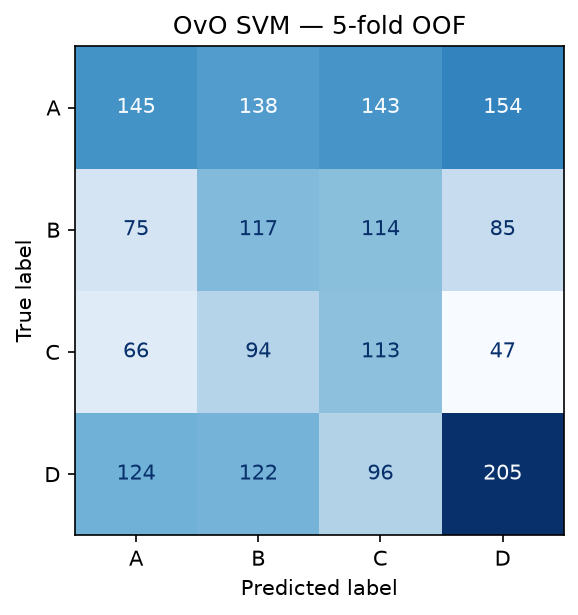
\includegraphics[width=\linewidth]{cm_ovo.png}\caption{OvO SVM}\end{subfigure}\hfill
\begin{subfigure}{0.32\textwidth}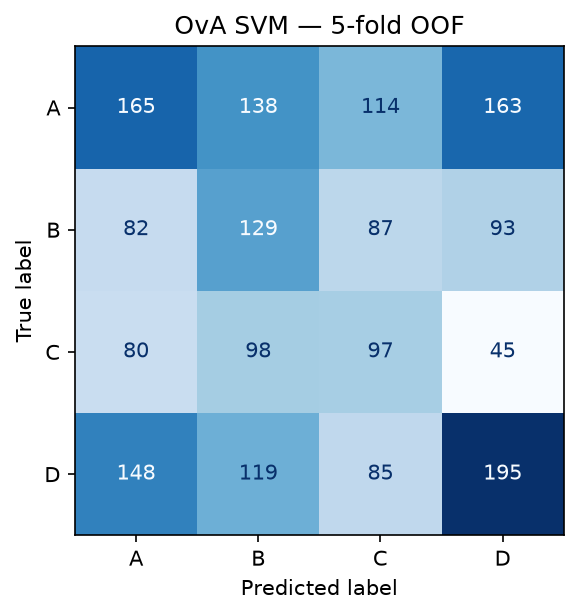
\includegraphics[width=\linewidth]{cm_ova.png}\caption{OvA SVM}\end{subfigure}\hfill
\begin{subfigure}{0.32\textwidth}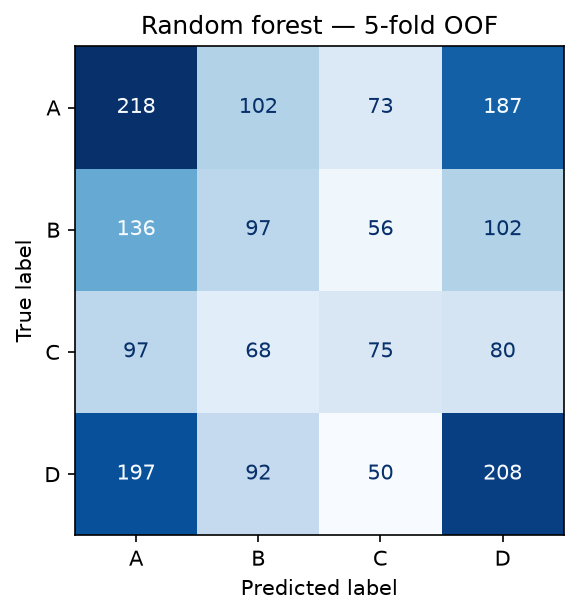
\includegraphics[width=\linewidth]{cm_rf.png}\caption{Random forest}\end{subfigure}
\caption{Confusion matrices of pooled 5-fold OOF predictions (rows = true, columns = predicted).}\label{fig:cm}
\end{figure}

\begin{table}[H]\centering\small
\caption{Per-class precision (P), recall (R) and F1 from pooled 5-fold OOF predictions.}\label{tab:prf}
\begin{tabular}{@{}lccccccccc@{}}
\toprule
& \multicolumn{3}{c}{OvO SVM} & \multicolumn{3}{c}{OvA SVM} & \multicolumn{3}{c}{Random forest} \\
\cmidrule(lr){2-4}\cmidrule(lr){5-7}\cmidrule(lr){8-10}
Class & P & R & F1 & P & R & F1 & P & R & F1 \\
\midrule
A & 0.3537 & 0.2500 & 0.2929 & 0.3474 & 0.2845 & 0.3128 & 0.3364 & 0.3759 & 0.3550 \\
B & 0.2484 & 0.2992 & 0.2715 & 0.2665 & 0.3299 & 0.2949 & 0.2702 & 0.2481 & 0.2587 \\
C & 0.2425 & 0.3531 & 0.2875 & 0.2533 & 0.3031 & 0.2760 & 0.2953 & 0.2344 & 0.2613 \\
D & 0.4175 & 0.3748 & 0.3950 & 0.3931 & 0.3565 & 0.3739 & 0.3605 & 0.3803 & 0.3701 \\
\midrule
Accuracy & \multicolumn{3}{c}{0.3156} & \multicolumn{3}{c}{0.3188} & \multicolumn{3}{c}{0.3254} \\
Macro-F1 & \multicolumn{3}{c}{0.3117} & \multicolumn{3}{c}{0.3144} & \multicolumn{3}{c}{0.3113} \\
Weighted-F1 & \multicolumn{3}{c}{0.3178} & \multicolumn{3}{c}{0.3208} & \multicolumn{3}{c}{0.3227} \\
\bottomrule
\end{tabular}
\end{table}

\paragraph{Most confused segments.} Counting errors in both directions, \textbf{A$\leftrightarrow$D} is the
most confused pair for every model (278 OvO, 311 OvA, 384 RF), followed by \textbf{A$\leftrightarrow$B}
(213, 220, 238). Third is A$\leftrightarrow$C for OvO (209) and B$\leftrightarrow$D for OvA (212) and
RF (194). Segment A, the largest, is part of the two most confused pairs for every model.
The three models are very close (macro-F1 0.311--0.314, accuracy 0.316--0.325). The RF is slightly
better on A and D; the SVMs have higher recall on C (0.353 OvO, 0.303 OvA vs.\ 0.234 RF). B and C
remain the hardest segments for all models (F1 0.26--0.29).

\subsection{(d) One-vs-one vs.\ one-vs-all}
On the paired OOF predictions: OvO accuracy 0.3156, OvA 0.3188, difference (OvO $-$ OvA)
$=-0.0033$. A paired bootstrap over rows (10{,}000 resamples) gives a \textbf{95\% CI of
$[-0.0169, +0.0103]$}, which contains 0. The models agree on 84.6\% of rows; among the 154 discordant
rows OvO alone is right on $b=74$ and OvA alone on $c=80$. The exact McNemar test (binomial on
$b$ out of $b+c$, $p_0=0.5$) gives \textbf{$p=0.6871$}. \textbf{The difference is not statistically
significant}, and macro-F1 is practically the same (0.3117 vs.\ 0.3144).

\paragraph{Choice.} We would choose \textbf{OvA} for this dataset. Its performance is statistically
indistinguishable from OvO (and nominally slightly higher), it needs only $K=4$ SVMs instead of 6, and it
produces one continuous score per segment that can be ranked or thresholded for targeting. Its main
weakness, the skew of each one-vs-rest problem, is handled by \texttt{class\_weight="balanced"}, which the
grid search selected. OvO would pay off with many classes or very large $n$ (each SVM trains on a small
subset), neither of which applies here.

\subsection{(e) Baselines and significance}
\begin{table}[H]\centering\small
\caption{Baselines vs.\ models (same folds; stratified baseline averaged over 20 seeds).}\label{tab:base}
\begin{tabular}{@{}lcc@{}}
\toprule
Model & Accuracy & Macro-F1 \\
\midrule
Majority class (always A) & 0.3156 & 0.1199 \\
Stratified random & 0.2662 & 0.2514 \\
OvO SVM & 0.3156 & 0.3117 \\
\textbf{OvA SVM (best by macro-F1)} & \textbf{0.3188} & \textbf{0.3144} \\
Random forest & 0.3254 & 0.3113 \\
\bottomrule
\end{tabular}
\end{table}

The best model by the selection metric is the OvA SVM, but the margin over RF (0.3113) and OvO
(0.3117) is far inside the fold std (about 0.02--0.03): the three are effectively tied.

\paragraph{Accuracy: one-sided binomial test} ($H_0$: accuracy $=0.3156$, the majority rate). OvA is
correct on 586/1838 = 0.3188, \textbf{$p=0.39$}, one-sided 95\% lower bound 0.3009: \emph{not
significant}. Likewise OvO (580/1838, $p=0.51$) and RF (598/1838 = 0.3254, $p=0.19$). The test
assumes independent trials, which CV and model selection only approximately satisfy.

\paragraph{Macro-F1: label-permutation test} (1{,}000 permutations; full pipeline refitted on the same
five folds for each permuted label vector). OvA macro-F1 0.3143 vs.\ permuted mean 0.2475 (max 0.2971),
\textbf{$p=0.001$}, the smallest attainable value; OvO (0.3113, perm.\ mean 0.2459, max 0.2875) and RF
(0.3109, perm.\ mean 0.2463, max 0.2889) also give $p=0.001$. \emph{Significant.}

\paragraph{Interpretation and practical significance.} The models have learned real, non-random
structure that lets them recognise all four segments (macro-F1 0.19 above the majority rule and 0.06
above stratified guessing; B and C recall 0.33 and 0.30 for OvA), but they do not get more rows right
than always guessing A: OvA is correct on only 6 more of 1{,}838 rows (+0.3 points). Practically the
improvement is small; roughly two of three predictions are wrong, so the predictions suit only cheap,
reversible decisions.

\paragraph{Advice to the sales team (141 words).}\leavevmode
\begin{center}
\fbox{\begin{minipage}{0.92\textwidth}\small
Treat the predicted segments for the 789 new customers as a weak hint, not a reliable label. Our best
model (one-vs-all SVM) is right about 32\% of the time, no better than always guessing the most common
segment A. It does pick up real patterns, so it spreads its guesses across all four segments more
sensibly than chance, but about two in three predictions will still be wrong. Use the predictions only
for low-cost choices, such as the order of first calls or which brochure to send first. Do not drop
customers or commit expensive campaigns based on the predicted segment. Confirm each customer's segment
during early contact and record it, so future models can learn from it. Collecting better information,
such as purchase intent, budget or income, and preferred vehicle type, would likely help more than a
more complex model.
\end{minipage}}
\end{center}

%=====================================================================
\section{Conclusion}
%=====================================================================
We built one-vs-one and one-vs-all classifiers from binary SVMs with order-independent tie-breaking,
and a random forest with our own bootstrap, aggregation and OOB estimate, all inside a leakage-free
preprocessing pipeline. Selection by macro-F1 led to RBF SVMs ($C=1$, $\gamma=0.1$, balanced weights)
and a 200-tree forest of unrestricted depth. On identical folds the three models are practically tied
(accuracy 0.316--0.325, macro-F1 0.311--0.314); OvO and OvA do not differ significantly (McNemar
$p=0.69$, bootstrap CI containing 0), and we prefer OvA for its simplicity and per-class scores.
All models beat chance in macro-F1 (permutation $p=0.001$) but not the majority rule in accuracy
(binomial $p=0.39$ for OvA). Only Age and Family\_Size have permutation importances clearly above zero. The available attributes explain little of
the sales team's segmentation, so the predictions for the 789 new customers should be used as a weak
prior and refined through direct contact and richer data.

\end{document}
